\chapter{Interactions entre compétition intraspécifique et température dans la
régulation des populations structurées}
\chaptermark{Compétition intraspécifique et température}
\label{chap:fip}

\vspace{2cm}
\begin{Spacing}{1}
\texttt{
Mallard, François, Vincent Le Bourlot, Christie Le Coeur, Monique Avnaim, David
Claessen and Thomas Tully, "From individuals to populations: \\intraspecific
competition breaks the temperature-size rule"\\
soumis à Journal of Animal Ecology}
\end{Spacing}
\vspace{2cm}


\lettrine[lines=3]{A}{u cours} des trois chapitres précédents, nous avons étudié
le rôle des mécanismes de compétition intraspécifiques sur la dynamique de
populations structurées de collemboles \textit{Folsomia candida} d'un point de vu théorique
et empirique. Ces études nous ont permis en particulier de mieux appréhender
l'impact de différents niveaux de compétition par interférence dans la
dynamique temporelle de la structure des populations. Cependant, ces études ont
été réalisées dans une seule condition environnementale. Hors, comme nous
l'avons déjà expliqué, l'environnement, et en particulier la température, peut
avoir un impact à la fois sur les individus et les populations. 

En effet, des températures différentes affectent directement les taux
physiologiques (métabolisme, consommation, respiration,\ldots), ce qui a des
conséquences démographiques via des changements dans les cycles de vie
\autocites{gillooly2002a,le-galliard2012a}. des changements de température
provoque aussi de la plasticité phénotypique chez les individus en modifiant par
exemple l'allocation des ressources à la croissance ou à la reproduction
\autocites{liefting2010temperature,gutteling2007mapping}. Ceci résulte notamment
dans la règle dite ``taille-température'' qui prédit une taille plus grande des
individus dans des environnements plus froids
\autocites{atkinson1994a,atkinson1996a,angilletta2009a}. Enfin, la température
peut également avoir un effet sur les comportements individuels comme
l'activité,la dispersion ou le choix de l'habitat
\autocites{atacho2013a,bonte2008thermal,vanbeest2012temperature}.

L'approche classique de l'étude de l'influence de la température sur les
phénotypes consiste à mesurer des normes de réaction \autocites{woltereck1909a}.
Ces mesures sont généralement réalisées sur des individus isolés ou sur de
petites cohortes élevées au laboratoire dans différentes conditions de
température. Ces analyses apportent beaucoup d'informations sur les effets au
niveau de l'individu mais laissent de côté les conséquences de ces effets aux
niveaux des populations et des communautés. 

Dans ce chapitre, nous nous demandons a quel point les normes de réactions
mesurées au niveau individuel permettent des inférences sur la dynamique des
populations. Nous cherchons à comprendre comment les effets directs de la
température sur les traits d'histoire de vie individuels sont modulés par les
interactions entre individus et les rétroactions démographiques.
Les effets d'une augmentation de la température sur la compétition
inter-spécifique ont déjà été démontrés, provoquant notamment une augmentation
de la compétition par exploitation. Mais le cas de la compétition
intra-spécifique reste peu clair, et les effets sur la compétition par
interférence peuvent être différents de l'exploitation. L'interaction entre
les deux mécanismes, couplés aux effets directes de la température sur les individus,
rendent l'impact de la température sur les dynamiques des populations
structurées difficile à prévoir. Pour y parvenir, nous avons mesuré les normes de réaction
individuelles des taux de croissance et des tailles à maturité et tailles
asymptotiques dans quatre conditions de température, $11$, $16$, $21$ et
$26\degres$C. Nous avons également effectué des mesures de taux de croissance de
cohortes et de taille des cohortes adultes dans des populations élevées aux même
températures. Nous avons ainsi pu comparer les réponses à la température dans
deux conditions démographiques contrastées et en déduire l'importance de la
compétition intra-spécifique dans la réponse des populations à la température.

\section{Éléments de méthodologie}

\subsection{Conditions d'élevages et mesures}

Comme dans les expériences précédentes, les conditions d'élevage et les méthodes
de mesure de la taille individuelle et de la structure des populations suivent
les descriptions données dans le Chapitre \ref{chap:method}.

\subsubsection{Individus isolés}

Les nouveaux nés sont isolés immédiatement après la naissance et sont nourris
\textit{ad libitum} pendant toute leur vie. Les individus ont été placé
aléatoirement à une des quatre températures de notre intervalle ($11$, $16$, $21$ et
$26\degres$C). La taille corporelle est mesurée pour chaque individu trois fois
par semaine pendant dix semaines, puis une fois par semaine. Afin de déterminer
la maturation des individus, les boites d'élevage sont régulièrement inspecter
pour rechercher des pontes. La croissance des individus est ensuite modélisée
par une fonction logistique ajustée sur les mesures de taille (Figure
\ref{fig:FIP1}).
Le taux de croissance maximal moyen et la taille asymptotique sont estimés par des modèles
de moindre-carrés non linéaire ajustés séparément pour chacune des trajectoires
de croissance \autocites{pinheiro2000a}. Les effets fixes du clone et de la
température, prise comme variable catégorielle, sur le taux de croissance
maximal et la taille asymptotique ont été testés à l'aide de modèles linéaires
et de test de Fisher.

\begin{figure}[!ht]
\begin{center}
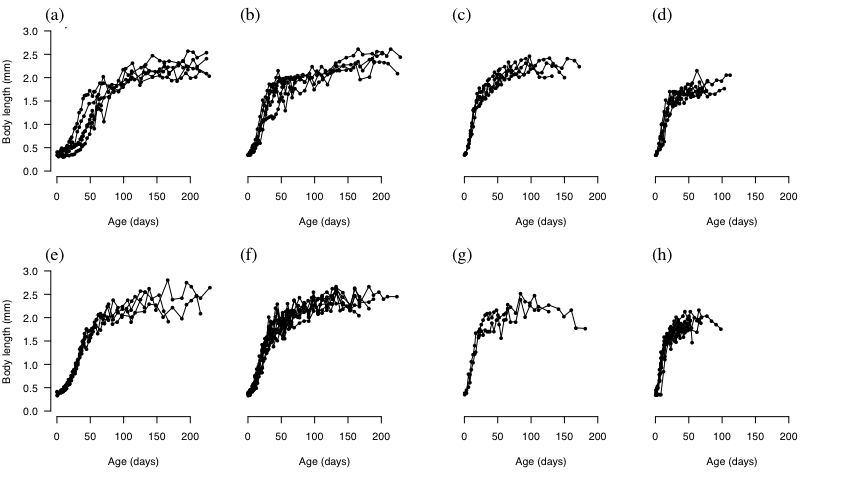
\includegraphics[width=\textwidth]{1_CorpsDeThese/Resumes/Fig/FIP01}
\caption[\lofimage{1_CorpsDeThese/Resumes/Fig/FIP01}Trajectoires de croissance
individuelles]{Trajectoires de croissance individuelles pour les clones HA
(a-d) et TO (e-h) à $11$ (a et e), 16 (b et f), 21 (c et g) et
$26\degres$C (d et h).}
\label{fig:FIP1}
\end{center}
\end{figure}

\begin{figure}[H]
\begin{center}
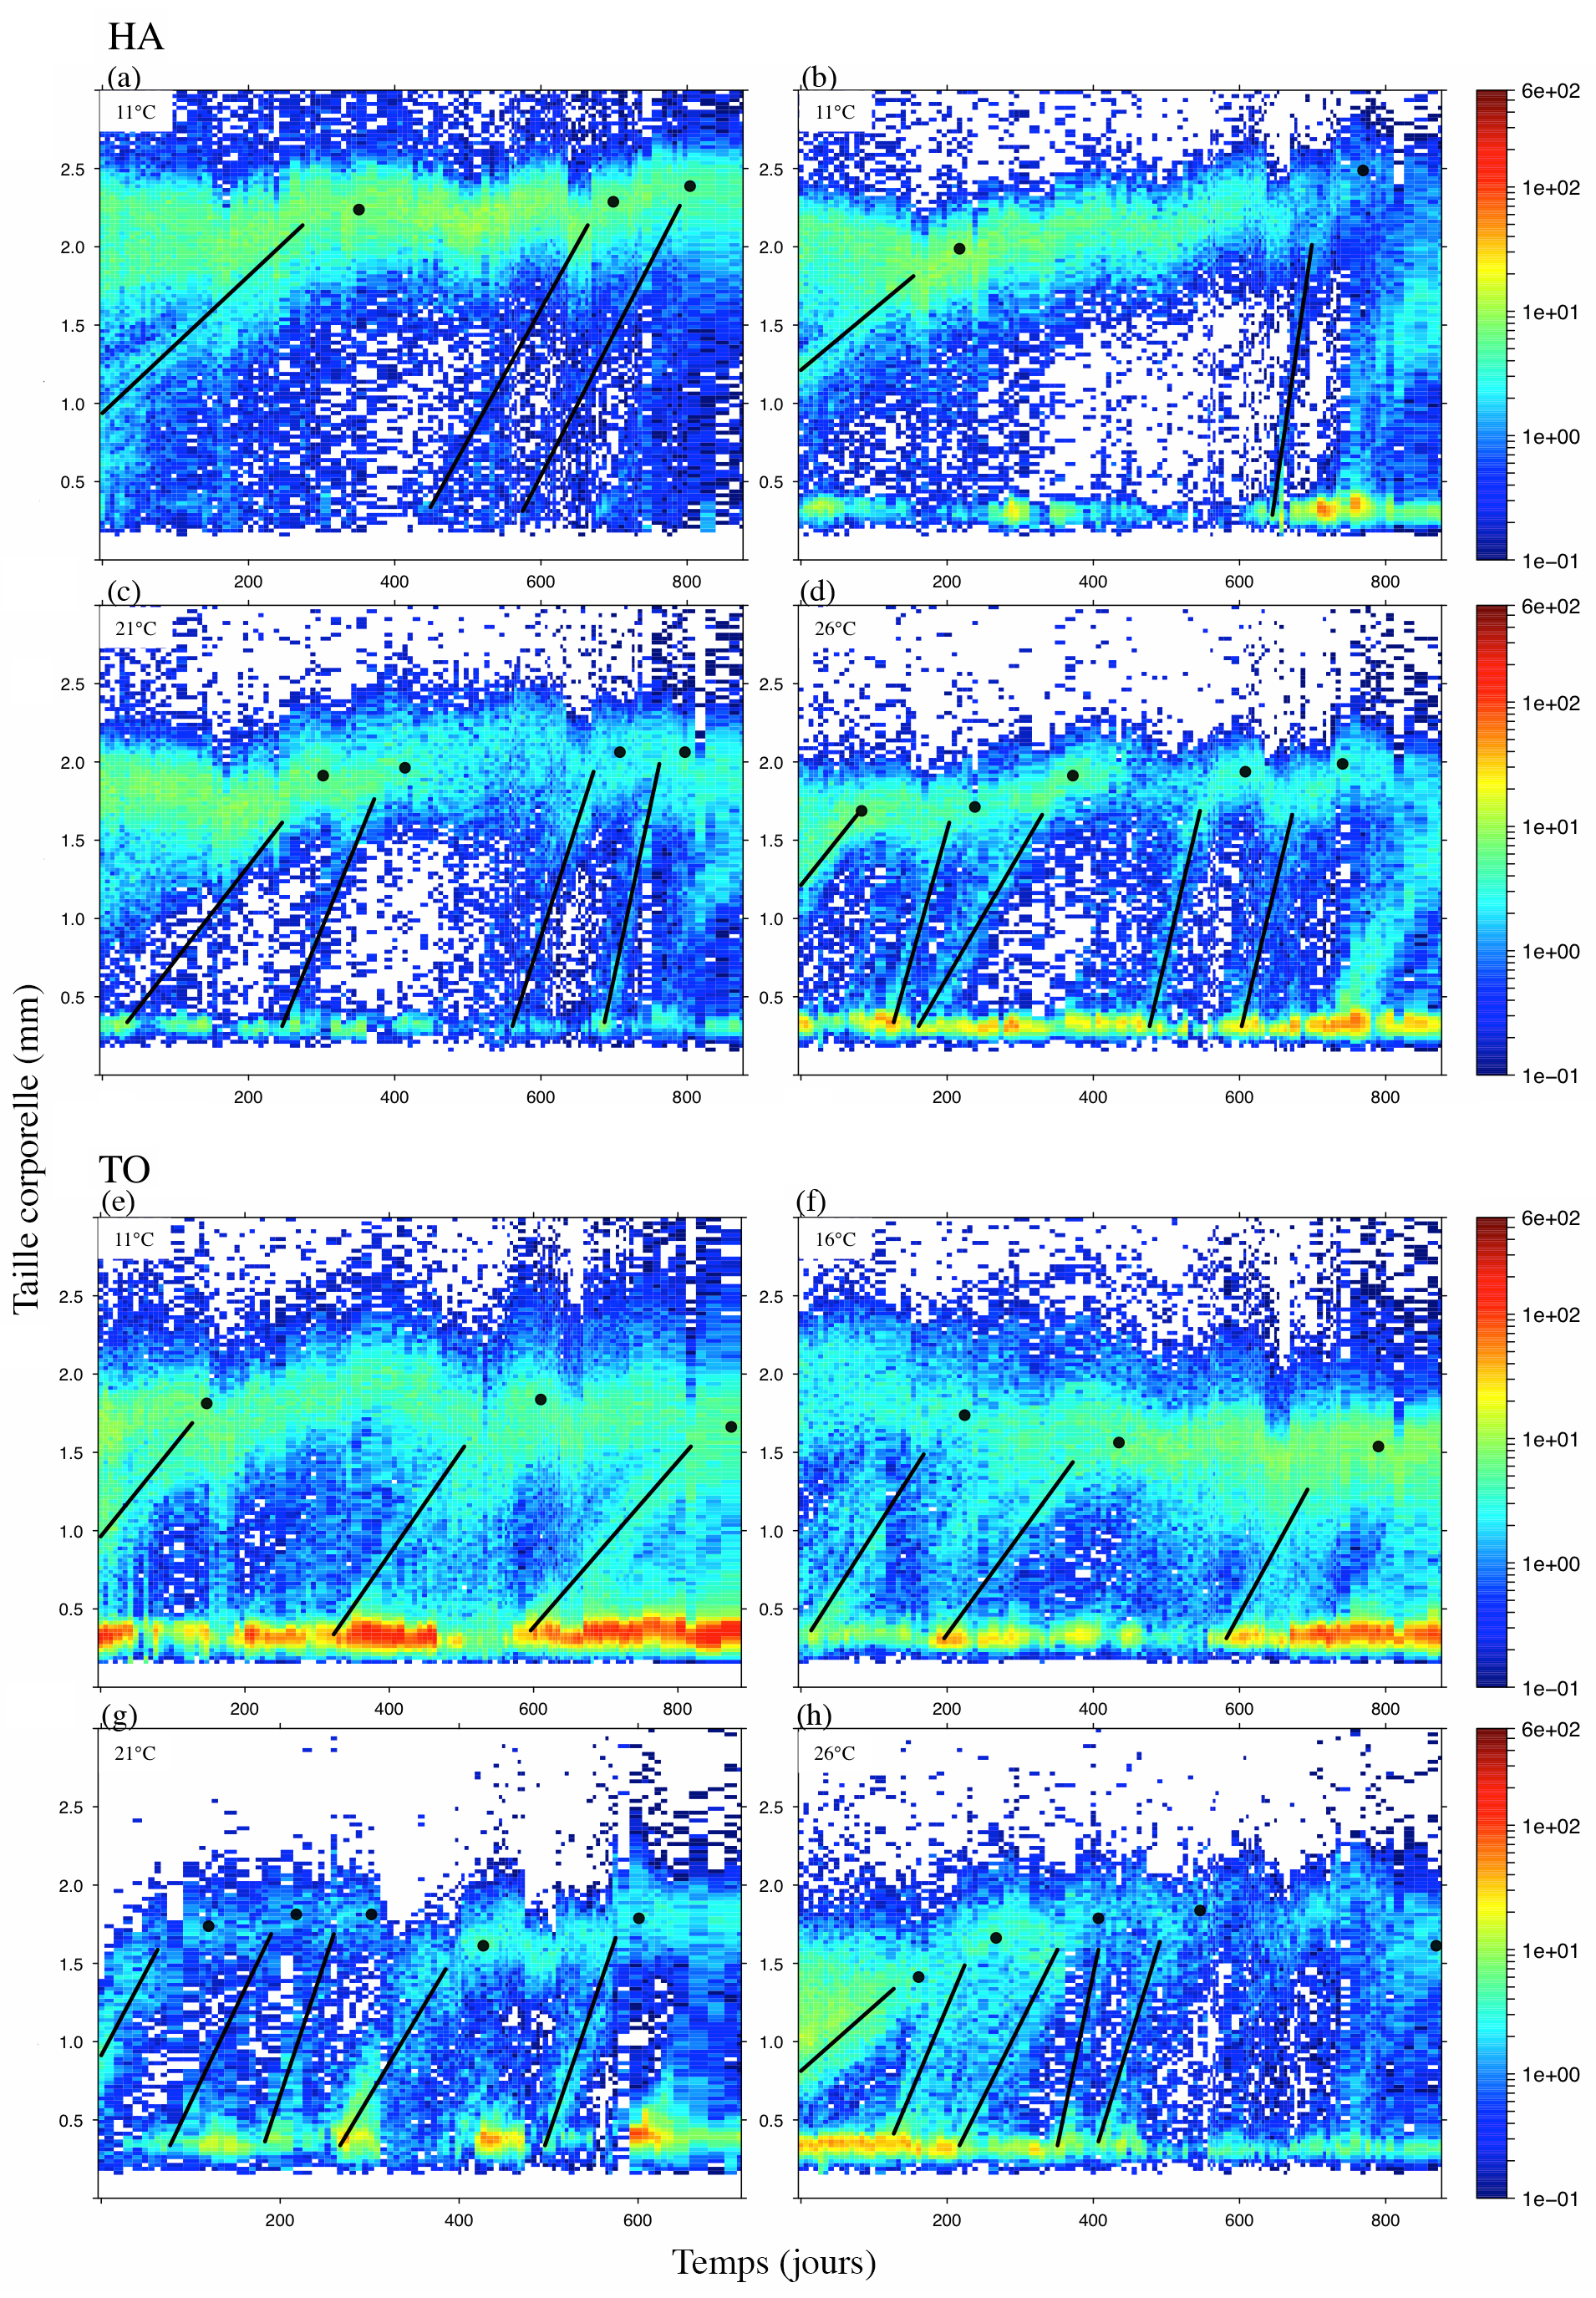
\includegraphics[width=\textwidth]{1_CorpsDeThese/Resumes/Fig/FIP02}
\caption[\lofimage{1_CorpsDeThese/Resumes/Fig/FIP02}Exemples de diagrammes
structures temps]{Exemples de diagrammes
structures temps pour les clones HA
(a-d) et TO (e-h) à $11$ (a et e), 16 (b et f), 21 (c et g) et $26\degres$C
(d et h). Les points noirs marquent les mesures de taille
adulte, tandis que les lignes marquent les mesures de
croissance de cohortes.}
\label{fig:FIP2}
\end{center}
\end{figure}

\subsubsection{Mesures de taille et de croissance dans les populations}

Pour les mesures de normes de réactions en contexte de population, quatre
populations ont été démarrées pour chaque température, excepté $21\degres$C où
les populations présentées dans le Chapitre \ref{chap:sp} sont utilisées. La
structure des populations a été mesurée une fois par semaine pendant plus d'un
an. Les traits d'histoire de vie (taux de croissance des juvéniles et taille
adulte) ont été extraits des données grâce à la représentation en diagramme
structure-temps et aux outils annexes présentés dans le Chapitre
\ref{chap:method} Section \ref{sec:stdiag}. 

Les taux de croissances juvéniles ont été mesurés sur des cohortes suffisamment
visibles sur les diagrammes et atteignant le groupe d'adultes (Figure
\ref{fig:FIP2}).
Le taux de croissance est estimé par la pente de la taille moyenne dans les cohortes au
cours du temps. La taille asymptotique des adultes est mesurée comme la taille
moyenne du groupe d'adultes une fois que la cohorte a totalement fusionné avec
les adultes déjà présents, ou quand sa taille moyenne se stabilise. La structure
de la population au moment de chaque mesure nous permet d'en connaître les
conditions démographiques (densité de juvéniles, d'adultes,\ldots). Les
individus sont considérés adultes lorsque leur taille excède $0.8mm$.

\subsubsection{Séparer les effets température et densité dépendance}

Dans nos populations, les changements dans les trais d'histoire de vie et les
taux démographiques peuvent être attribué à des effets directs de la température
sur les individus, à des effets directs des mécanismes de densité dépendance, ou
à une interaction entre les deux. Afin de pouvoir analyser les effets de la
densité dépendance (éventuellement en interaction avec la température) tout en
contrôlant pour les effets directs de la température, nous avons construit deux
indicateurs qui comparent les traits mesurés dans les populations aux mesures
faites sur les individus isolés. 

Pour analyser les différents effets sur le taux de croissance, nous avons
utilisé des modèles linéaires expliquant le rapport des taux de croissance dans
les populations sur les taux maximum moyens mesurés chez les individus isolés.
Nous appelons cet indicateur le ``\textbf{taux de croissance relatif en
population}''. Les variables explicatives que nous avons considéré sont le
logarithme du nombre d'adultes, la température, la lignée clonale et les
interactions entre les trois variables. 

De la même façon, nous avons étudié la taille des adultes dans les populations
en la comparant aux mesures effectuées sur les individus isolés. Plus
précisément, nous avons construit un indicateur que nous appelons
``\textbf{l'effort de croissance au delà de la maturité}'' ($GEBM$: ``Growth
Effort Beyond Maturation''). Cet indicateur représente l'investissement dans la
croissance après avoir atteint la maturité en conditions de populations comparé
à l'investissement en isolation. Il dépend de la température et se calculs comme
la proportion de croissance au delà de la taille à maturité (mesurée en isolation) comparée à la taille
maximum mesurée en isolation:

\begin{equation}
GEBM(T) = \frac{Taille\ adulte_{populations}(T) -
Taille\ \grave{a} \ maturit\acute{e}_{isolation}(T)}{Taille\ adulte_{isolation}(T) -
Taille\ \grave{a} \ maturit\acute{e}_{isolation}(T)}
\end{equation}

A une température donnée, la taille à maturation et la taille maximum étant
connue pour les individus élevées en isolation, le $GEBM$ nous indique à quel
point un individu continue de croître après la maturation: $GEBM=0$ signifie que
les adultes stoppent leur croissance après la maturation, $GEBM=50\%$ qu'ils
atteignent une taille à mi-chemin de la taille asymptotique en isolation. Des
valeurs inférieures à 0 ou supérieures à $100\%$ signifie respectivement que les
adultes grandissent moins que la taille moyenne à maturité en isolation, ou
qu'ils grandissent plus que la taille maximum moyenne en isolation. N'ayant pas
trouvé de différence significative entre les deux clones, toutes les valeurs de
$GEBM$ ont été regroupées pour les analyses. Nous avons construit des modèles
linéaires avec comme variables explicatives la densité d'adultes, la
température et la lignée clonale avec toutes les interactions possibles. La
significativité des effets a été mesurées à l'aide d'ANOVA et de tests de
Fisher.

\section{Résultats}

\subsection{Normes de réactions à la température}

\subsubsection{Taux de croissance}

\begin{figure}[!ht]
\begin{center}
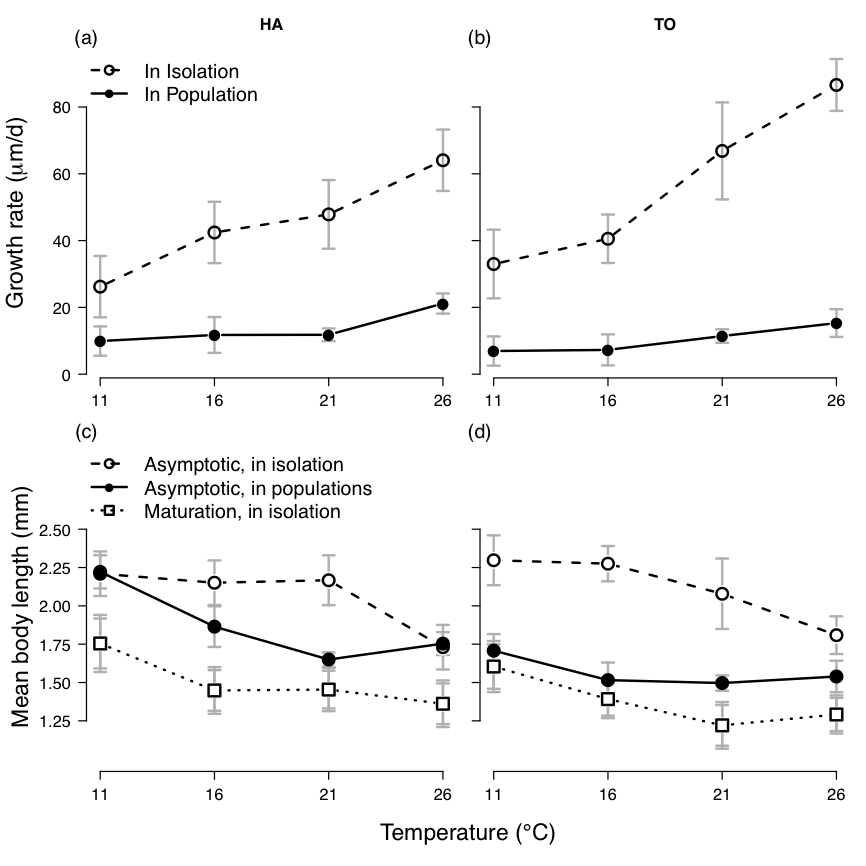
\includegraphics[width=0.95\textwidth]{1_CorpsDeThese/Resumes/Fig/FIP03}
\caption[\lofimage{1_CorpsDeThese/Resumes/Fig/FIP03}Normes de réactions des taux
de croissance et tailles moyennes]{Normes de réactions des taux de croissance (a
et b, moyennes et intervalles de confiance à $95\%$) pour les clones HA (a) et TO (b) mesurés en isolation (tirets) et sur les cohortes en condition de population (lignes pleines). Normes
de réaction de la taille corporelle (c et d): taille moyenne à maturité
(pointillés) et taille asymptotique des individus isolés (tirets) comparés à la
taille adulte moyenne en populations (lignes pleines).}
\label{fig:FIP3}
\end{center}
\end{figure}

La Figure \ref{fig:FIP3} représente les taux de croissance et les différentes
tailles mesurées en isolation ou en population pour les deux clones. On peut
observer qu'en isolation, le taux de croissance individuel augmente quasiment
linéairement avec la température chez les deux clones (Figure \ref{fig:FIP3}a
et b). A $11\degres$C, les taux de croissance ne sont pas différents entre HA et
TO. Mais le taux de croissance augmente plus vite avec
la température chez TO que chez HA. Il en résulte à
$26\degres$C un taux de croissance $25\%$ supérieur chez TO par rapport à HA. 

Dans les populations, les taux de croissance mesurés sont beaucoup plus faibles
qu'en isolation (Figure \ref{fig:FIP3}a et b). En moyenne, il semble que les
juvéniles du clone HA grandissent plus vite que ceux de TO, mais l'effet de la
température sur les taux de croissance est le même pour les deux clones. 

\subsubsection{Tailles à maturité et taille asymptotique}

Chez les deux clones, les individus isolés suivent quasiment les mêmes normes de
réaction à la température, que ce soit pour la taille asymptotique ou pour la
taille à maturité (Figure \ref{fig:FIP3}c et d). Comme prédit par la règle
taille-température, la taille asymptotique diminue avec la température pour les
deux clones, sans différence significative entre eux. De plus, à part à
$11\degres$C où HA mature légèrement plus grand que TO, la taille à maturité
diminue avec la température de façon similaire pour les deux clones. 

Contrairement aux individus isolés, l'effet de la température sur la taille
moyenne des adultes en condition de population est différent pour les deux
clones. A $11\degres$C, les cohortes du clone HA atteignent en population une
taille qui n'est pas significativement différente de la taille asymptotique en
isolation (Figure \ref{fig:FIP3}c). Puis cette taille adulte moyenne décroît
progressivement pour être proche de la taille à maturité à une température de $21\degres$C. Mais de façon
beaucoup plus étonnante, la taille moyenne des adultes dans les populations du
clone HA ré-augmente entre 21 et $26\degres$C. 

Chez le clone TO à $11$ et $16\degres$C, les cohortes dans les populations
s'arrêtent de grandir peu de temps après avoir atteint leur taille à maturité
attendu d'après les mesures en isolations. Entre $16$ et $26\degres$C, la taille
moyenne des adultes reste statistiquement constante à une valeur intermédiaire
entre la taille à maturité et la taille asymptotique mesurées en isolation
(Figure \ref{fig:FIP3}d).

\subsection{Densité dépendance et température}

Pour comprendre les différences entre les normes de réaction mesurées sur les
individus isolés et sur les cohortes en populations, nous avons étudier la
réponse à la température et à la densité de nos deux indicateurs, le taux de
croissance relatif et le $GEBM$, et ce pour les deux lignées clonales. Nous
avons utilisé la densité d'adultes dans les populations comme mesure de densité
car les adultes représentent en moyenne $90\%$ de la biosurface totale des
populations, et nous avons pu démontrer leur rôle prépondérant dans la dynamique
des populations structurées (voir Chapitres \ref{chap:sp} à \ref{chap:sm}). 

\subsubsection{Taux de croissance relatif}

\begin{figure}[!ht]
\begin{center}
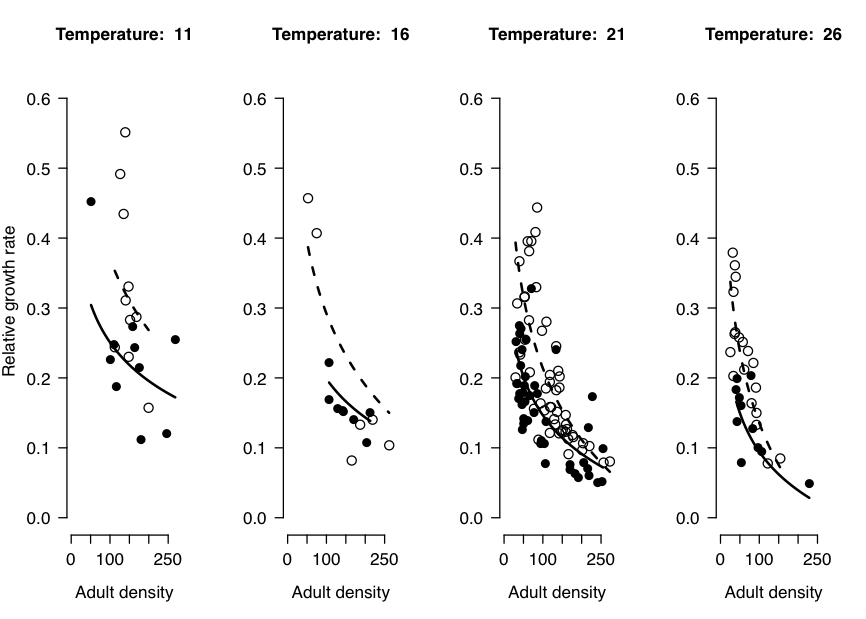
\includegraphics[width=\textwidth]{1_CorpsDeThese/Resumes/Fig/FIP04}
\caption[\lofimage{1_CorpsDeThese/Resumes/Fig/FIP04}Taux de croissance
relatifs]{Taux de croissance relatifs en fonction de la densité d'adultes dans
les populations pour les clones HA (lignes tiretées et symboles ouverts) et TO
(lignes pleines et symboles pleins)}
\label{fig:FIP4}
\end{center}
\end{figure}

A chaque température, le taux de croissance des cohortes de juvéniles dans les
populations diminue avec la densité d'adulte en suivant u.e loi exponentielle
(Figure \ref{fig:FIP4}, Table \ref{tab:FIP1}). En moyenne, les juvéniles des
populations du clone HA grandissent plus vite que ceux du clone TO, mais l'effet
délétère de la densité d'adulte y est également plus fort. Les différences
génétiques entre les clones ont donc tendance à s'atténuer avec la densité. 

\begin{table}
\centering
\caption{\label{tab:FIP1}Résultats du modèle pour le taux de croissance relatif
des cohortes de juvéniles dans les populations.}
\scriptsize
\begin{tabular}{rccccl}
\hline 
\multicolumn{6}{c}{$lm(\text{taux de croissance} \sim (\log(\text{Densité
d'adultes}) + \text{Température}) * \text{Clone})$} \\
&&&&&\\
& Estimation & Erreur standard & Valeur $t$ & $\text{Pr}(>|t|)$ & \\
\hline

Intercepte = Clone HA, Température 11 & $1.22e+00$ & $8.59e-02$ & $1.42e+01$
& $<2e-16$ & $***$\\

$\log(\text{Densité d'adultes})$ & $-1.48e-01$ & $1.34e-02$ & $-1.10e+01$ & $<
2e-16$ & $***$\\

$\text{Température}$ & $-1.57e-02$ & $1.82e-03$ & $-8.60e+00$ & $8.61e-15$ & $***$\\

$\text{CloneTO}$ & $-4.90e-01$ & $1.18e-01$ & $-4.15e+00$ & $5.56e-05$ & $***$\\

$\log(\text{Densité d'adultes}):\text{CloneTO}$ & $6.79e-02$ & $1.86e-02$ & $3.65e+00$ &
$3.61e-04$ & $***$\\

$\text{Température}:\text{CloneTO}$ & $5.24e-03$ & $2.63e-03$ & $2.00e+00$ &
$4.79e-02$ & $*$\\

\hline 
\end{tabular} 
\end{table}

L'augmentation de la température a également tendance à réduire le taux de
croissance relatif des cohortes. Cet effet est légèrement plus intense pour HA,
mais c'est probablement du à un taux de croissance plus élevé que TO à faible
densité. 

\subsubsection{Effort de croissance après maturation}

\begin{figure}[!ht]
\begin{center}
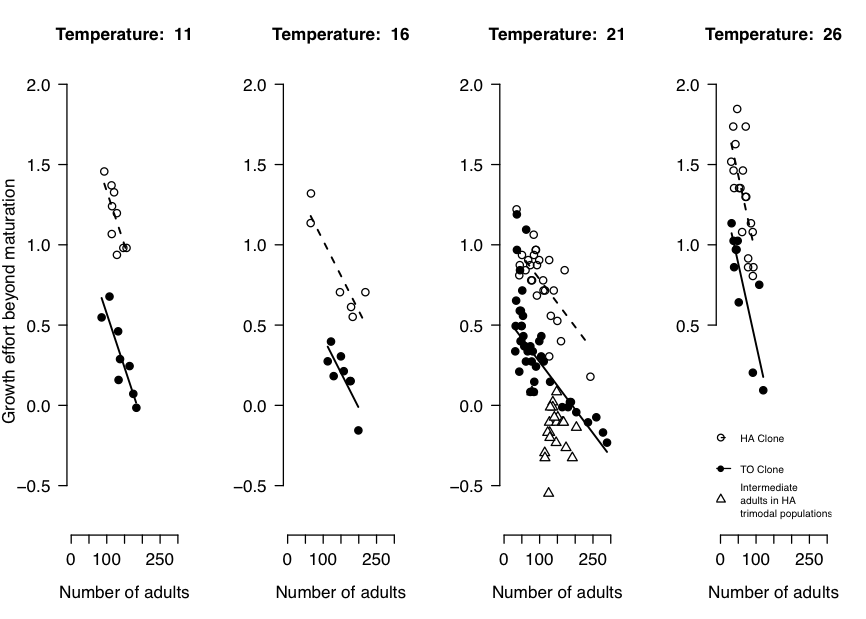
\includegraphics[width=\textwidth]{1_CorpsDeThese/Resumes/Fig/FIP05}
\caption[\lofimage{1_CorpsDeThese/Resumes/Fig/FIP05}GEBM]{Effort de croissance
après maturité ($GEBM$) en fonction de la densité d'adultes pour les quatre
températures. }
\label{fig:FIP5}
\end{center}
\end{figure}

La plupart des populations étudiées possèdent une structure bimodale similaire à
celles décrites dans le Chapitre \ref{chap:sp}. Cela permet de discriminer les
adultes des juvéniles (voir Supplementary Materials de l'Annexe \ref{Ann:fip})
et ainsi d'estimer la densité et la taille moyenne des adultes afin d'estimer le
$GEBM$. La Figure \ref{fig:FIP5} montre que les réponses du $GEBM$ à la
densité et à la température diffèrent quantitativement mais pas qualitativement
entre les deux lignées (voir aussi Table \ref{tab:FIP2}). En moyenne, le $GEBM$
de HA est supérieur à celui de TO, indépendamment de la température. Cependant,
les différences entre clones s'atténuent avec la température. Pour chaque clone,
le $GEBM$ est négativement corrélé à la densité d'adulte: plus la densité
d'adultes est grande, plus leur taille moyenne se rapproche de la taille à
maturité mesurée sur les individus isolés à la même température. La pente de
cette corrélation et la même pour les deux clones à chaque température et donne
une mesure de la dépendance à la densité. 

\begin{table}
\centering
\caption{\label{tab:FIP2}Résultats du modèle pour le taux de croissance relatif
des cohortes de juvéniles dans les populations.}
\scriptsize
\begin{tabular}{rccccl}
\hline 
\multicolumn{6}{c}{$lm(GEBM \sim (\text{Densité
d'adultes} + \text{Clone}) * \text{Température})$} \\
&&&&&\\
& Estimation & Erreur standard & Valeur $t$ & $\text{Pr}(>|t|)$ & \\
\hline

Intercepte = Clone HA, Temperature11 & $2,01E+00$ & $1,93E-01$ & $1,04E+01$ & $<
2e-16$ & $*** $\\
Température16 & $-5,43E-01$ & $2,43E-01$ & $-2,23E+00$ & $2,77E-02$ & $* $\\
Température21 & $-9,25E-01$ & $1,98E-01$ & $-4,68E+00$ & $8,18E-06$ & $*** $\\
Température26 & $-7,06E-02$ & $2,10E-01$ & $-3,37E-01$ & $7,37E-01$ & $ $\\
Densité d'adultes & $-6,72E-03$ & $1,50E-03$ & $-4,48E+00$ & $1,84E-05$ & $*** $\\
CloneTO & $-7,62E-01$ & $7,88E-02$ & $-9,68E+00$ & $< 2e-16$ & $*** $\\
Densité d'adultes:Temperature16 & $2,35E-03$ & $1,77E-03$ & $1,33E+00$ & $1,87E-01$ & $ $\\
Densité d'adultes:Temperature21 & $3,76E-03$ & $1,53E-03$ & $2,46E+00$ & $1,56E-02$ & $* $\\
Densité d'adultes:Temperature26 & $-3,34E-03$ & $1,91E-03$ & $-1,75E+00$ & $8,36E-02$ & $. $\\
Température16:CloneTO & $1,58E-01$ & $1,15E-01$ & $1,37E+00$ & $1,73E-01$ & $
$\\
Température21:CloneTO & $2,48E-01$ & $8,80E-02$ & $2,82E+00$ & $5,71E-03$ & $**
$\\
Température26:CloneTO & $2,13E-01$ & $9,93E-02$ & $2,15E+00$ & $3,39E-02$ & $*
$\\

\hline 
\end{tabular} 
\end{table}

Comme observé au cours du Chapitre \ref{chap:sp}, certaines populations du clone
HA à $21\degres$C exhibent une structure trimodale avec deux groupes d'adultes
stabilisés à des tailles différentes. Nous pouvons dès lors calculer le $GEBM$
indépendamment pour les deux groupes d'adultes.
Dans ces populations, nous avons trouvé un $GEBM$ très différents pour les deux groupes d'adultes. Alors que les adultes
les plus grands ont un $GEBM$ qui suit le même modèle général que pour les
autres populations, le $GEBM$ des adultes les plus petits n'est pas expliqué par
le nombre total d'adultes dans les populations. Nous n'avons pas non plus trouvé
de corrélation significative entre le nombre d'adultes de petite taille et leur
$GEBM$. En revanche, à la fois le nombre d'adultes de petite taille et leur
taille moyenne sont corrélés au nombre d'adultes de plus grande taille. Nous
avons donc modélisé le $GEBM$ de tous les groupes d'adultes du clone HA à
$21\degres$C à l'aide du nombre d'adultes de plus grande taille (ou du nombre
total d'adultes pour les structures bimodales). Il est intéressant de constater
qu'il n'y a alors pas de différence significative dans la pente de la régression
entre le $GEBM$ des adultes de grande taille et celui des plus petits,
seulement dans leur intercepte. Dans les populations trimodales, la présence d'adultes de
grande taille agit donc sur le $GEBM$ plus petits de la même façon que si les
populations étaient bimodales avec des petits adultes, mais en densité
supérieure ($260$ adultes de plus, voir Figure \ref{fig:FIP6}).

\begin{figure}[!ht]
\begin{center}
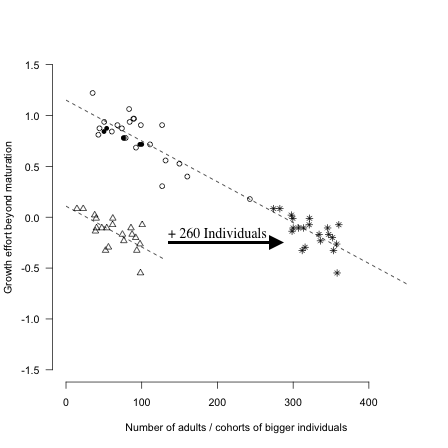
\includegraphics[width=0.75\textwidth]{1_CorpsDeThese/Resumes/Fig/FIP06}
\caption[\lofimage{1_CorpsDeThese/Resumes/Fig/FIP06}GEBM dans les
populations HA à $21\degres$C]{GEBM dans les
populations HA à $21\degres$C pour les adultes de petite taille ($\triangle$) et
de grande taille ($\circ$) dans les populations trimodales, et pour les petits
adultes s'il y avait 260 petits adultes de plus à la place des grands ($\ast$).}
\label{fig:FIP6}
\end{center}
\end{figure}

\subsubsection{Normes de réaction à la température des indicateurs}

L'indicateur $GEBM$ dépend également de la température pour nos deux lignées
clonales. Cependant, contrairement au taux de croissance relatif, l'effet de la
température sur $GEBM$ n'est pas linéaire. Afin d'étudier l'effet de la
température sur nos deux indicateurs en contrôlant pour l'effet de la densité au
sein de chacun des clones, nous avons tracé les taux de croissance relatifs et
$GEBM$ prédits pour une densité de 100 adultes en utilisant les modèles ajusté
pour chaque lignée indépendamment (Figure \ref{fig:FIP7a}). 

\begin{figure}[!ht]
\begin{center}
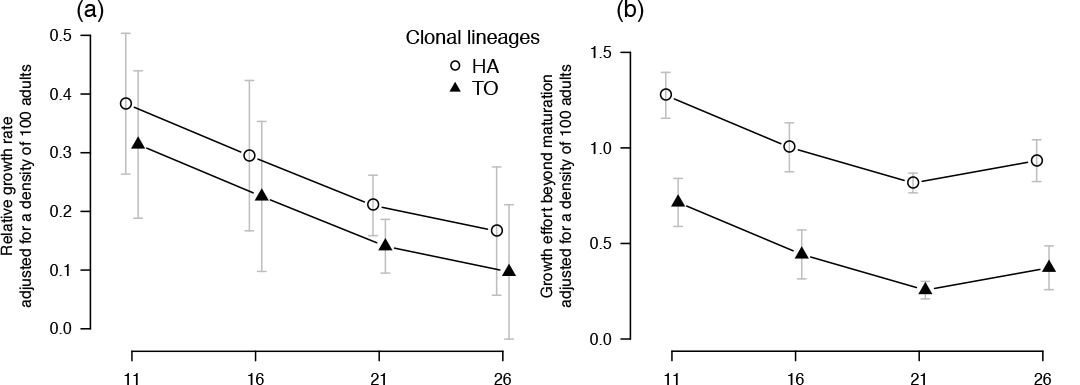
\includegraphics[width=0.75\textwidth]{1_CorpsDeThese/Resumes/Fig/FIP07a}
\caption[\lofimage{1_CorpsDeThese/Resumes/Fig/FIP07a}Normes de réaction
prédites à la température]{Normes de réacions à la température prédites pour
une densité de 100 adultes. (a) Taux de croissance relatif. (b) Effort de
croissance après maturation.}
\label{fig:FIP7a}
\end{center}
\end{figure}

Dans les deux lignées génétiques, le taux de croissance relatif décroît
linéairement avec la température (Figure \ref{fig:FIP7a}a), mais la norme de
réaction de $GEBM$ suit une forme en U: $GEBM$ décroît entre $11$ et
$21\degres$C mais augmente ensuite jusqu'à $26\degres$C (Figure
\ref{fig:FIP7a}b). Cette augmentation à la température la plus chaude testée est
remarquable car dans la plupart des populations élevées à $26\degres$C, la
taille adulte moyenne est plus grande que la taille asymptotique mesurée sur les
individus isolés à la même température (Figure \ref{fig:FIP6}cd), alors qu'à
$21\degres$C chez HA, certaines cohortes n'atteignent pas la taille à maturité
mesurée en isolation (Figure \ref{fig:FIP6}c, valeurs négatives).

\section{Discussion}

\subsection{Normes de réaction des individus isolés}

Les normes de réactions mesurées sur des individus isolés montrent que les
Collemboles de l'espèce \textit{Folsomia candida} suivent la règle dite
``taille-température'' \autocites{atkinson1994a,angilletta2009a}. En effet,
dans des conditions froides, les individus grandissent plus lentement mais
atteignent des tailles supérieures à des individus isolés élevés dans des
conditions plus chaudes \autocites{angilletta2003a}. Bien que des études aient
déjà montré des effets similaires de la température sur les taux de croissance
de collemboles juvéniles \autocites{birkemoe2000a, driessen2007a, ellers2008a,
ellers2011b} ou sur la taille à maturité \autocites{stam1996a}, cette étude est
à notre connaissance la première à démontrer expérimentalement un ajustement
plastique de la taille adulte à différentes conditions de température ambiante.
Malgré des stratégies démographiques différentes entre les deux clones étudiés
\autocites{tully2008a,tully2011a}, les différences génétiques entre les clones
n'entraînent que très peu de différence dans les normes de réaction
individuelles à la température de la taille adulte, ce qui est similaire à ce
qui a déjà été observé chez un autre Collembole \autocites{driessen2007a}.

\subsection{Densité dépendance dans les populations}

Cette étude expérimentale constitue à notre connaissance la première description
expérimentale quantitative de dynamiques de populations structurées en taille le
long d'un gradient de température relativement large. Ces populations ont
généralement une structure bimodale avec un mode d'adultes et un mode de
juvéniles distincts. La plupart du temps, les juvéniles ne montrent pas de
croissance visible, mais un groupe de juvéniles parvient périodiquement à
grandir et recruter chez les adultes 

Que ce soit pour les taux de croissance ou les taille adultes, les normes de
réactions à la température en conditions de population sont différentes de
celles mesurées sur les individus isolés, avec des valeurs en moyenne plus
basses en population, probablement à cause de la compétition à l'oeuvre pour
l'accès aux ressources (voir les Chapitres précédents). Dans nos populations,
l'apport de ressource est le même quelque soit la température ambiante. Les
populations atteignent donc un équilibre dynamique où la quantité de ressource
disponible limite le nombre, la taille corporelle et l'investissement
reproductif des adultes. Les équilibres atteints par les populations résultent
de rétroactions complèxes entre des stratégies démographiques
\autocites[dépendantes des clones,][]{tully2008a,stam1996a} et les effets de la
densité dépendance \autocites{kokko2007a} qui proviennent principalement de deux
mécanismes: la compétition pour la nourriture et pour l'espace. 

Comme montré dans les Chapitres précédents, la compétition pour la nourriture
est un des facteurs principaux de régulation de la dynamique de
nos populations de Collemboles. Cette compétition régule également les taux de
croissance des cohortes de juvéniles et les tailles corporelles atteintes par
les adultes (voir Chapitres \ref{chap:sp}, \ref{chap:amnat} et \ref{chap:sm}).
Les effets négatifs de la densité sont visibles à deux échelles: (i) en
comparant les traits mesurés en populations aux traits mesurés sur des individus
isolés; et (ii) en comparant les traits mesurés dans des populations avec
différentes densités d'adultes. Nous avons montré dans cette étude que l'effet
négatif de la densité sur les traits d'histoire de vie peut être très fort (les
taux de croissance en population n'atteignent par exemple que 20 à $30\%$ des
valeurs mesurées sur des individus isolés). Cet effet de densité prend alors le
pas sur la plupart des ajustements plastiques dont les individus sont capables à
différentes températures. 

La comparaison des deux clones étudié a permis de mettre en évidence des
différence génétiques significatives dans l'intensité de la densité dépendance:
pour les deux traits étudiés, le clone HA souffre d'avantage d'une augmentation
de la densité d'adultes que le clone TO, et cela à toutes les températures
testées. Ces réponses différentes à la densité pourraient provenir d'une
différence génétique dans la sensibilité des juvéniles à la densité d'adultes
ou dans le niveau de compétition que les adultes imposent aux juvéniles. Afin de
discriminer entre ces deux hypothèse, on pourrait envisager une expérience où
l'on mesurerait les taux de croissance et les tailles atteintes par les juvéniles
de chaque clone élevés en présence d'adultes des deux clones. 

\subsection{Normes de réaction en population}

Le long du gradient de température testé, nous avons constaté que la plasticité
phénotypique observable chez les individus isolés était annulée voir inversée en
condition de population. Les interactions compétitives que les individus
subissent dans les populations suffisent à réduire fortement les taux de
croissance des juvéniles qui sont alors quasiment constants aux différentes
températures. Cependant, en comparant ces taux de croissance à ceux des
individus isolés et en contrôlant pour la densité, nous avons pu montrer un
effet négatif de la température: l'effet négatif de la densité sur les taux de
croissance est donc amplifié lorsqu'on augmente la température. Cela suggère que
l'intensité de la compétition subie par les juvéniles dans nos populations
augmente avec la température, ce qui est cohérent avec l'augmentation des taux
physiologiques à haute température \autocites{gillooly2001a}.

La taille moyenne des adultes dans les populations est elle aussi négativement
corrélée à la densité. Entre 11 et $21\degres$C, la diminution du $GEBM$ avec la
température montre que la taille moyenne des adultes dans les populations tend à
se rapprocher de la taille à maturité mesurée sur les individus isolés. De plus,
l'augmentation de la température provoque l'augmentation des taux de
consommation de la ressource alors même que l'apport de nourriture reste
constant. Des résultats théoriques ont montré que dans ces conditions,
l'augmentation de la température amplifie l'avantage compétitif des plus jeunes
lié à leur plus grande efficacité dans la gestion de l'énergie
\autocites{ohlberger2011a}.
De plus, d'après les modèles de populations physiologiquement structurées, cet
avantage compétitif dans le cas de l'exploitation fait converger la taille
maximale atteinte par les adultes vers la taille à maturité. Ainsi, la
diminution du $GEBM$ entre 11 et $21\degres$C pourrait être due à une
augmentation avec la température de l'intensité de la compétition par
exploitation. 

Cependant, au delà de $21\degres$C, on observe la tendance inverse avec une
augmentation du $GEBM$. Cela ne peut pas être expliqué par une plus faible
densité, ni par un effet direct de la température sur les individus.
Ceci laisse donc entendre que l'augmentation de la par exploitation avec la
température n'est pas le seul phénomène responsable des effets de la densité
dépendance dans nos populations. Alors que l'augmentation de la compétition par
exploitation tends à avoir des tailles adultes proches de la taille à maturité,
une augmentation de la compétition par interférence provoque l'émergence
d'individus de très grande taille (voir Chapitre \ref{chap:amnat}). L'importance
relative des deux types de compétition pourrait donc être à l'origine de la
réponse plastique de la taille adulte dans les populations. Alors que la
compétition par exploitation est probablement dominante à faible température du
fait de l'activité réduite des individus, si la compétition par interférence
augmente plus rapidement avec la température que la compétition par
exploitation, elle pourrait finir par dominer à partir d'une certaine
température et rendre possible l'apparition de grands individus malgré une
température élevée, tel que proposé sur la Figure \ref{fig:FIP7b}.

\begin{figure}[!ht]
\begin{center}
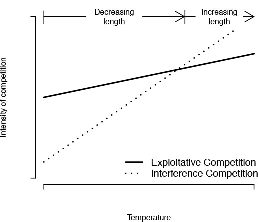
\includegraphics[width=0.75\textwidth]{1_CorpsDeThese/Resumes/Fig/FIP07b}
\caption[\lofimage{1_CorpsDeThese/Resumes/Fig/FIP07b}Importance relative
des différentes formes de compétitions]{Importance relative
des différentes formes de compétitions avec la température et leurs effets sur
la taille des adultes en condition de population.}
\label{fig:FIP7b}
\end{center}
\end{figure}

Les résultats présentés sur les populations HA trimodales montrent également que
la cohorte d'individus les plus grands imposent la densité et la taille de la
cohorte d'adultes plus petits. Ceci démontre encore une fois le rôle de la
compétition par interférence dans la régulation de nos populations, où un
adulte de grande taille reproduits les effets de densité dépendance produits par
quatre adultes de petite taille. La taille des plus grands adultes étant environ
deux fois supérieure à celle des adultes les plus petits dans les populations
trimodales, ce facteur d'environ 4 apporte un argument venant appuyer
l'hypothèse de la densité ressentie par les individu dépendante de la longueur
au carré dans le modèle présenté dans le Chapitre \ref{chap:amnat}, eq.
\refeq{eq_an2} page \pageref{eq_an2}.

Les mécanismes par les quels la température agit sur la compétition par
interférence ne sont cependant pas clairs. Nous avons montré dans le Chapitre
\ref{chap:sm} que les individus les plus grands empêchaient les plus petits
d'accéder à la ressource. Nous pensons que l'augmentation de la température, en
augmentant les taux métaboliques et l'activité augmentent à la fois la fréquence
à la quelle les collemboles sont en besoin de nourriture (2 fois par cycle de
vie, \citealp{palevody1974a}) alors que l'apport reste constant, et la fréquence
des interaction directes entre les individus, augmentant de ce fait l'intensité
de la compétition par interférence. 

La forme en U des normes de réactions de $GEBM$ pourraient donc être dues à
l'augmentation simultanée de la compétition par exploitation et par
interférence, mais avec des vitesse différentes (Figure \ref{fig:FIP7b}). En
dessous d'une température critique, bien qu'augmentant moins vite, la
compétition par exploitation reste la force régulatrice majeure de la dynamique
des populations, et l'augmentation de la température provoque alors une
diminution de la taille adulte qui tend vers la taille à maturité. Au delà de la
température critique, la compétition par interférence devient dominante, et
l'augmentation de la température, en augmentant l'intensité de l'interférence,
favorise finalement des individus de grande taille. Dans ce cadre, l'existence
de populations trimodales à $21\degres$C, décrites dans les chapitre précédents,
pourrait être expliquée par des compétitions par exploitation et par
interférence relativement équilibrées qui ainsi permettrait l'émergence de
grandes individus mais ne permettrait pas l'arrêt complet de la croissance des
juvéniles qui pourraient quand même maturer et s'arrêter de grandir à une taille
adulte intermédiaire. Ceci constitue donc une autre hypothèse complémentaire à
celle des conditions initiales pour l'apparition de ces populations trimodales.
En effet, bien qu'aillant des conditions initiales identiques, seules certaines
populations à $21\degres$C ont atteint des structures trimodales, jamais aux
auters températures. 

\section{En conclusion}

En mesurant des traits d'histoire de vie à la fois sur des individus isolés et
dans des populations, nous avons pu montrer que: (i) les effets de la densité
dépendance peuvent l'emporter sur les effets de la température attendus d'après
les mesures sur les individus isolés; et (ii) les effets de la densité
dépendance subissent eux-mêmes des changements liés aux conditions de
température. Ceci montre l'importance d'identifier clairement les différentes
composantes de la densité dépendance (compétition par exploitation ou
interférence par exemple) et leur réponses à la température afin d'être capable
de prédire les réactions des populations aux changements de température en cours
et à venir. 
